\documentclass[conference, onecolumn]{IEEEtran}
\IEEEoverridecommandlockouts
\usepackage{cite}
\usepackage{amsmath,amssymb,amsfonts}
\usepackage{graphicx}
\usepackage{textcomp}
\usepackage{float}
\usepackage{tikz}
\usetikzlibrary{arrows.meta,positioning,fit}

\begin{document}

\title{Smart Locker with Anomalous Access Detection Based on IoT Device Telemetry}

\author{
1\textsuperscript{st} Duc Hoang Nguyen, 2\textsuperscript{nd} Viet Tien Nguyen, 3\textsuperscript{rd} Huy Hoang Nguyen,\\ 4\textsuperscript{th} Thanh Cao Nguyen, and Vo Minh Thu Le\\
FPT University, Ho Chi Minh Campus, Vietnam\\
\{duchoang.nguyen103, tiennguyen100306, huyhoang.ct06, thanhcao19112006\}@gmail.com, and thulvm@fpt.edu.vn}
\maketitle

\begin{abstract}
Shared campus lockers are usually opened with a key or a paper code, cannot be reserved in advance, and give staff no
view of forced openings, lost cards or items left for days; once networked, their open signal can also be spoofed.
SmartLocker is a web-based locker rental system: users reserve a slot on an online map, pay from a prepaid wallet, and
open it with a per-booking PIN, an RFID card, a fingerprint or a phone page. The ESP32 box never decides; it forwards
every credential to the server, which answers \texttt{UNLOCK} or \texttt{DENY}. Abnormal access is detected in two
tiers: a priority-ordered rule engine over device telemetry and server data recognises sensor faults, spoofed remote
opens, lost cards, forced opening, wrong-user access, items left behind and overdue storage, and a machine-learning risk
score raises an alert only when no rule matches. On 480 synthetic, labelled telemetry sessions, the best of four Weka
classifiers (k-nearest neighbours) reached a weighted F1 of 0.977 in 10-fold cross-validation. Most of its errors are
between wrong-user and normal sessions, which the data generator builds from the same formulas; this illustrates why
identity is checked by a rule, not by telemetry. The system passed all 66 unit and integration tests and all 472 API
test assertions (18 scenarios). Six replayed detection scenarios gave the expected labels (two after
adjusting the simulator), and on localhost the server answered device requests in a mean time of 6--31~ms per endpoint.
\end{abstract}

\begin{IEEEkeywords}
Smart locker, Internet of Things, ESP32, RFID, anomaly detection, rule engine, machine learning, Weka.
\end{IEEEkeywords}

\section{Introduction}

Self-service lockers are widely used for parcels and short-term storage on campuses, in canteens, gyms and libraries
\cite{iwan2016parcel}. Simple lockers, however, rely on a mechanical key or a code shared on paper, cannot be reserved
in advance, and leave staff blind to what happens at the box: a forced door, a lost card used by someone else or items
left for days are noticed only when someone complains. Connecting the locker to a server through the Internet of Things
(IoT) \cite{alfuqaha2015iot} solves the visibility problem but adds new risks: a device can be impersonated, an
``open'' signal can be forged, and sensor data can be wrong or tampered with \cite{sicari2015security}.

SmartLocker, developed as a course project at FPT University, addresses both sides. Its main functions are:
\begin{itemize}
  \item \textbf{Rental.} Users find a free slot on a map, book and pay from a prepaid wallet, open the slot with a PIN,
        an RFID card, a fingerprint or a phone page, and can cancel or extend; overdue items are locked in and charged,
        never released. Every money and time rule runs inside a database transaction.
  \item \textbf{Thin, authenticated box.} The ESP32 box forwards every credential to the server with a per-device secret
        key and opens only on the server's \texttt{UNLOCK}.
  \item \textbf{Abnormal access detection.} A priority-ordered rule engine over box telemetry and server data, plus a
        machine-learning risk score for cases no rule describes; lockouts, offline detection, overdue escalation and a
        hash-chained audit log cover what is visible from the server's own state.
\end{itemize}
We verify the system with automated tests, replayed detection scenarios, server-side response times, and a comparison
of four classifiers that illustrates, on synthetic data in which wrong-user and normal sessions share the same
telemetry, that telemetry alone does not separate
wrong-user from normal access. Section~II reviews related work, Section~III
presents the architecture and hardware, Section~IV the detection method, Section~V the implementation, Section~VI the
results, and Section~VII concludes.

\section{Related Work}

\textbf{Smart and parcel lockers.} Parcel lockers have been studied mainly as a last-mile delivery solution, where they
reduce failed deliveries and courier travel \cite{iwan2016parcel}. These works focus on logistics efficiency rather
than on access security or on the behaviour of the people who use the lockers.
A recent RFID--IoT locker \cite{rfidiot2023locker} authenticates the user with the unique identity card, and uses Wi-Fi
connectivity for continual status monitoring, storage of login and logoff data, and surveillance of unauthorised
access. SmartLocker builds on the same idea of a networked, card-authenticated locker, and adds what a shared locker
service needs on top of it: online reservation on a map with prepaid payment, several credentials (PIN, card,
fingerprint and phone), and a two-tier detector that raises typed alerts (Section~IV) instead of only logging access.

\textbf{IoT security.} Surveys of IoT security point out that constrained devices are exposed to impersonation,
spoofed messages and physical tampering, and that authentication and trust must be handled carefully at the server
side \cite{sicari2015security}. RFID in particular is vulnerable to cloning, replay and relay attacks
\cite{mitrokotsa2010rfid}. SmartLocker follows this advice by keeping the box free of decisions: the box only forwards
credentials, and the server identifies the box by a secret key whose hash is stored in the database.

\textbf{Anomaly detection.} Anomaly detection techniques are commonly divided into rule-based, statistical and
machine-learning approaches \cite{chandola2009anomaly}. In intrusion detection, Sommer and Paxson
\cite{sommer2010outside} warn that machine-learning detectors are hard to interpret and produce costly false alarms,
and that they work best when the problem is narrow and well understood. Public IoT telemetry datasets such as TON\_IoT
\cite{moustafa2021toniot} have been released to evaluate such detectors. Following this line of work, SmartLocker uses
explicit rules for the cases that can be described precisely, and keeps the learned model as a secondary signal.

\textbf{Tools.} The classifiers are trained with Weka \cite{hall2009weka}; the audit log follows the hash-chaining idea
of Haber and Stornetta \cite{haber1991timestamp}; passwords are stored with BCrypt \cite{provos1999bcrypt}.

\section{System Architecture}

\subsection{Overview}

SmartLocker follows a three-tier architecture (Fig.~\ref{fig:arch}). Clients are web browsers (end users and staff),
the phone unlock page, and the ESP32 locker box. The application tier is a Java 8 Servlet/JSP application (MVC2) on
Apache Tomcat~9. The data tier is a SQL Server database, which also holds the business rules as stored procedures.

\begin{figure}[H]
\centering
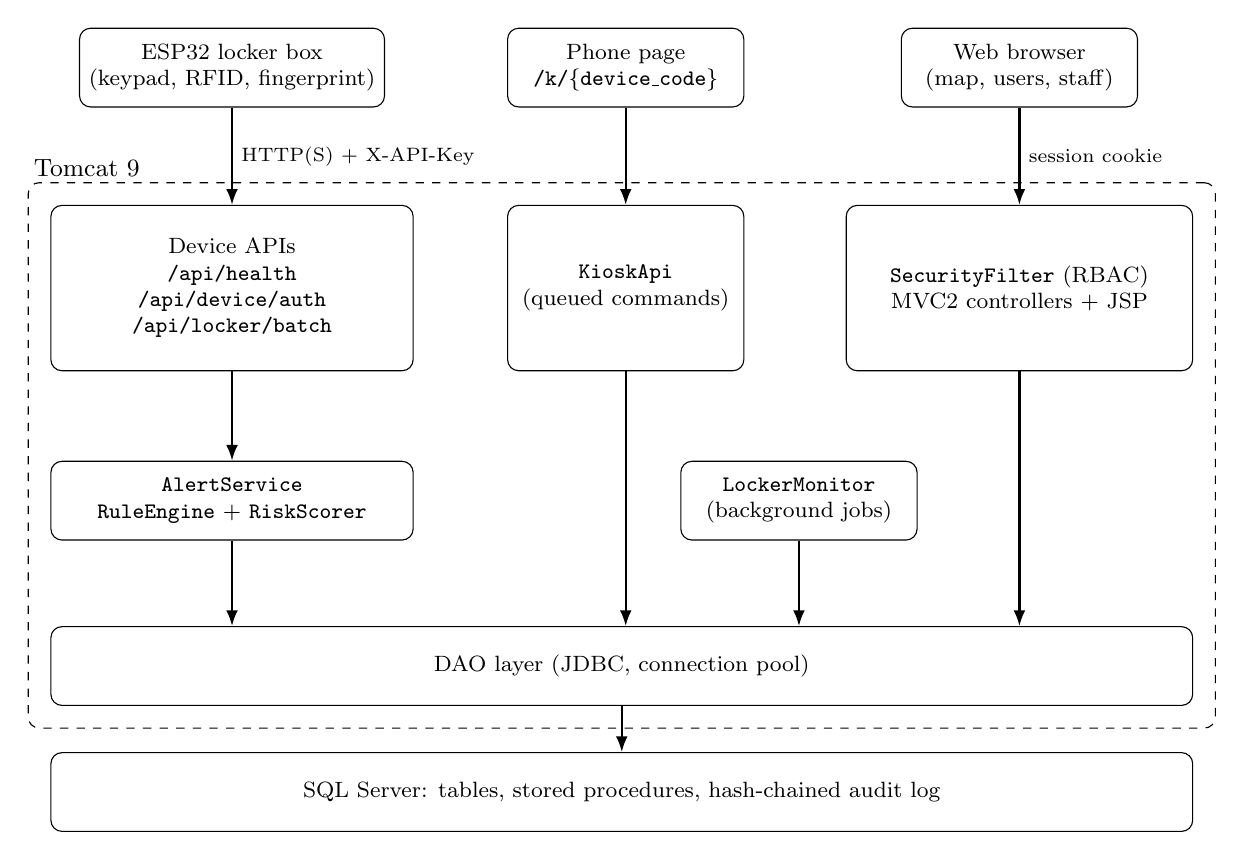
\begin{tikzpicture}[
  box/.style={draw, rounded corners, align=center, minimum height=1.0cm, minimum width=3.0cm, font=\footnotesize},
  tall/.style={box, minimum height=2.1cm},
  arr/.style={-{Latex[length=2mm]}, thick},
  lbl/.style={font=\scriptsize, align=left, inner sep=3pt}]
  \node[box] (esp)   at (0,4.6)  {ESP32 locker box\\(keypad, RFID, fingerprint)};
  \node[box] (phone) at (5,4.6)  {Phone page\\\texttt{/k/\{device\_code\}}};
  \node[box] (web)   at (10,4.6) {Web browser\\(map, users, staff)};
  \node[tall, minimum width=4.6cm] (devapi) at (0,1.8)  {Device APIs\\\texttt{/api/health}\\\texttt{/api/device/auth}\\\texttt{/api/locker/batch}};
  \node[tall, minimum width=3.0cm] (kiosk)  at (5,1.8)  {\texttt{KioskApi}\\(queued commands)};
  \node[tall, minimum width=4.4cm] (ctrl)   at (10,1.8) {\texttt{SecurityFilter} (RBAC)\\MVC2 controllers + JSP};
  \node[box, minimum width=4.6cm] (svc) at (0,-0.9)   {\texttt{AlertService}\\\texttt{RuleEngine} + \texttt{RiskScorer}};
  \node[box, minimum width=3.0cm] (mon) at (7.2,-0.9) {\texttt{LockerMonitor}\\(background jobs)};
  \node[box, minimum width=14.5cm] (dao) at (4.95,-3.0) {DAO layer (JDBC, connection pool)};
  \node[box, minimum width=14.5cm] (db)  at (4.95,-4.6) {SQL Server: tables, stored procedures, hash-chained audit log};
  \draw[arr] (esp)   -- node[lbl, right] {HTTP(S) + X-API-Key} (devapi);
  \draw[arr] (phone) -- (kiosk);
  \draw[arr] (web)   -- node[lbl, right] {session cookie} (ctrl);
  \draw[arr] (devapi) -- (svc);
  \draw[arr] (svc)   -- (svc |- dao.north);
  \draw[arr] (kiosk) -- (kiosk |- dao.north);
  \draw[arr] (ctrl)  -- (ctrl |- dao.north);
  \draw[arr] (mon)   -- (mon |- dao.north);
  \draw[arr] (dao)   -- (db);
  \node[draw, dashed, rounded corners, fit=(devapi)(kiosk)(ctrl)(svc)(mon)(dao), inner sep=8pt,
        label={[font=\small, anchor=south west, inner sep=2pt]north west:Tomcat 9}] {};
\end{tikzpicture}
\caption{System architecture of SmartLocker.}
\label{fig:arch}
\end{figure}

\subsection{Roles and Functions}

The web application serves five roles through role-based access control: \textbf{END\_USER} (book, pay, open, extend,
cancel, top up), \textbf{OPERATOR} (remote open, top-up approval, areas, banks, slots, plans, cards, bookings),
\textbf{TECHNICIAN} (alerts, maintenance tickets, sensor calibration), \textbf{AUDITOR} (read-only, verifies the audit
chain) and \textbf{ADMIN} (everything, including roles and permissions). Visitors may view the locker map without signing
in; every other page and every write request requires a session. Lockers are organised as \emph{areas} (shown as pins
on a map drawn with Leaflet, or with Mapbox GL when a Mapbox access token is configured), \emph{banks} (a column of lockers managed by one device) and \emph{slots} of three sizes: S
($20\times20\times20$~cm), M ($40\times40\times40$~cm) and L ($60\times60\times60$~cm).

\subsection{Hardware}

The locker box is built around an ESP32 development board (Table~\ref{tab:hw}, Fig.~\ref{fig:hw}). A 4$\times$4 keypad
reads PINs and menu keys, a PN532 NFC reader reads RFID cards and also acts as an NFC tag for phones, an AS608 sensor reads fingerprints, a 16$\times$2 I$^2$C LCD
shows messages, and two servos drive the bolt and the door. An SRF05 ultrasonic sensor detects a person in front of the
box and only switches the LCD backlight. The box sends a heartbeat every 3~s and executes the commands returned with it.

\begin{table}[H]
\renewcommand{\arraystretch}{1.3}
\centering
\caption{Hardware Components of the Locker Box}
\label{tab:hw}
\begin{tabular}{l l l}
\hline
\textbf{Component} & \textbf{Function} & \textbf{ESP32 pins} \\
\hline
ESP32 Dev Module & Controller, Wi-Fi, HTTP(S) client & -- \\
PN532 & RFID card reader (I$^2$C, 0x24) & SDA 21, SCL 22 (shared with LCD) \\
AS608 & Fingerprint sensor (UART) & TX$\rightarrow$35, RX 15 \\
LCD 1602 I$^2$C & User messages & SDA 21, SCL 22 \\
Keypad 4$\times$4 & PIN and menu input & Rows 13, 14, 25, 26; columns 33, 19, 23, 27 \\
Servo (bolt) & Locks the slot & 32 \\
Servo (door) & Opens the door & 2 \\
SRF05 & Presence detection (backlight) & TRIG 5, ECHO 18 \\
\hline
\end{tabular}
\end{table}

\begin{figure}[H]
\centering
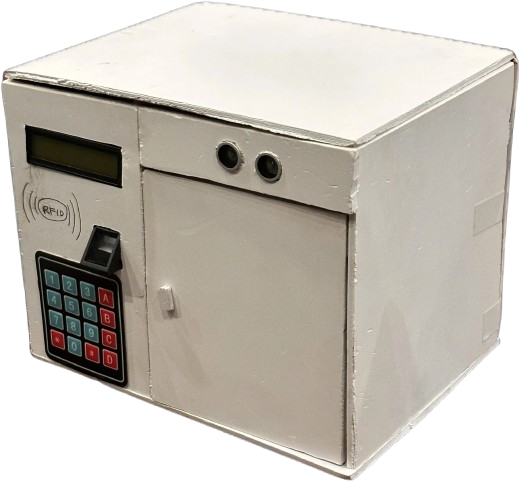
\includegraphics[width=0.45\linewidth]{images/hardware-box.png}
\caption{The assembled locker box prototype.}
\label{fig:hw}
\end{figure}

\subsection{Device Protocol}

Each box owns a secret API key; the database stores only its SHA-256 hash, and the server derives the device identity
from the key, never from the request body. The device API has three main endpoints (two more enroll a card or a
fingerprint):
\begin{itemize}
  \item \texttt{POST /api/health} -- heartbeat (every 3~s); the reply carries pending commands (remote \texttt{UNLOCK},
        fingerprint deletion) and the list of blocked card UIDs.
  \item \texttt{POST /api/device/auth} -- forwards a PIN, a card UID or a fingerprint slot with an \emph{intent}
        (\texttt{ASK}, \texttt{OPEN}, \texttt{CHECKOUT}); the server answers \texttt{UNLOCK}, \texttt{CHOOSE},
        \texttt{CONFIRM\_EMAIL} or \texttt{DENY} with a reason and the number of attempts left.
  \item \texttt{POST /api/locker/batch} -- uploads buffered access sessions (telemetry) with a per-device sequence
        number, so that a session re-sent after a network outage is stored only once.
\end{itemize}
The prototype firmware uses the first two endpoints and the enrollment ones; it does not upload sessions yet, so the
batch upload is exercised only by the device simulator (Section~VI).
One physical box may manage several banks. The \texttt{UNLOCK} reply carries a \texttt{physical} flag: the servo moves
only for the slot that is physically wired; for the other slots the LCD only confirms the operation.

A card can be read by anyone who finds it, so a card scan is confirmed by its owner when the server can send e-mail
and the owner has a real address (the seeded demo accounts skip this step). The box then receives
\texttt{CONFIRM\_EMAIL} and nothing opens: the server holds an \texttt{UNLOCK} command for 5~minutes and e-mails a
single-use link, of which it stores only the SHA-256 hash. The command is released when the owner confirms with a POST
on that link (a GET changes nothing, because mail scanners open links) or on the map while signed in, and the box takes
it with its next heartbeat, as for a phone open. A card scanned at a box that does not hold its booking is refused
with \texttt{WRONG\_PLACE}, which names the right bank.

The same PN532 also lets a phone open a slot without any card. Between two card polls it emulates an NFC tag that holds
the link \texttt{/k/\{device\_code\}?n=\{token\}}. The token comes from the server in the heartbeat reply
(\texttt{tap\_path}), changes every minute and after each use, and is accepted for 5~minutes. A phone that taps the box
opens that page; the signed-in owner presses ``open my locker'', which posts the token to \texttt{/api/kiosk/unlock}
(a GET changes nothing). The server checks the login and the token, so the box never learns who the phone belongs to,
and a token read from a photo or an old link is refused with \texttt{TAP\_EXPIRED}. The command then reaches the box
with its next heartbeat, as for any phone open.

\subsection{Booking Lifecycle}

A booking moves through the states in Fig.~\ref{fig:state}. A reservation charges the wallet and holds the slot for
15~minutes. A cancel within 5~minutes refunds 100\%, and a later cancel during the hold refunds 50\%; a cancel is possible
only during the hold. The first successful authentication at the box is
\texttt{CHECK\_IN}: the booking becomes \texttt{ACTIVE} and its due time starts. A reservation nobody checked in
when the hold ends checks in by itself (\texttt{AUTO\_CHECK\_IN}): the slot stays locked for its owner, nothing is
refunded, and the paid time counts from the end of the hold, so the owner may come early, late or never. If the slot
was never opened by the due time plus the grace time, nothing is inside to protect: the booking ends as a no-show, the
slot is free again and no late fee is charged; three such no-shows within 7~days block new bookings for a while. Later authentications make the box ask
``A: open / B: return'': key A opens the slot and keeps the rental (\texttt{ACCESS}), key B ends it (\texttt{PICKUP}).
A booking can be extended up to three times.

An overdue booking is never released automatically, because the user's belongings are still inside. After the grace
period the slot is \emph{locked}, every late hour is charged at 150\% of the hourly rate and the wallet may become
negative; the box then refuses to open (\texttt{OVERDUE\_UNPAID}) until the debt is paid. After 48~hours the booking is
escalated to staff with an \texttt{OVERDUE\_ESCALATED} alert.

\begin{figure}[H]
\centering
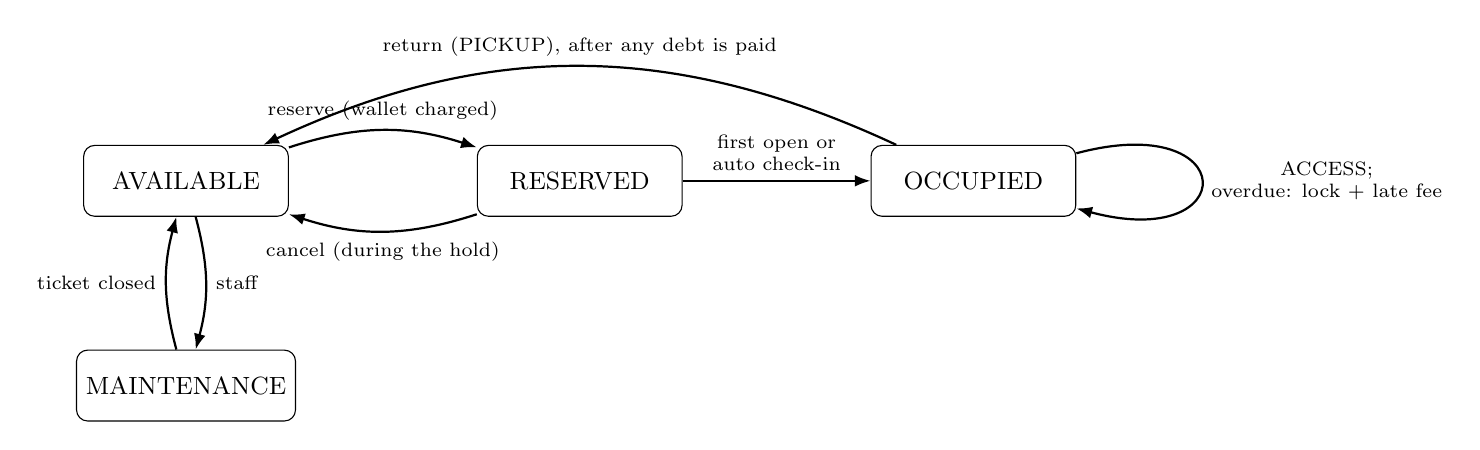
\begin{tikzpicture}[
  st/.style={draw, rounded corners, minimum width=2.6cm, minimum height=0.9cm, font=\small},
  arr/.style={-{Latex[length=2mm]}, thick},
  lbl/.style={font=\scriptsize, align=center}]
  \node[st] (av)  at (0,0)    {AVAILABLE};
  \node[st] (re)  at (5,0)    {RESERVED};
  \node[st] (oc)  at (10,0)   {OCCUPIED};
  \node[st] (mt)  at (0,-2.6) {MAINTENANCE};
  \draw[arr] (av) to[bend left=18] node[lbl, above] {reserve (wallet charged)} (re);
  \draw[arr] (re) to[bend left=18] node[lbl, below] {cancel (during the hold)} (av);
  \draw[arr] (re) -- node[lbl, above] {first open or\\auto check-in} (oc);
  \draw[arr] (oc) to[bend right=25] node[lbl, above] {return (PICKUP), after any debt is paid} (av);
  \draw[arr] (oc) to[loop right] node[lbl, right] {ACCESS;\\overdue: lock + late fee} (oc);
  \draw[arr] (av) to[bend left=15] node[lbl, right] {staff} (mt);
  \draw[arr] (mt) to[bend left=15] node[lbl, left] {ticket closed} (av);
\end{tikzpicture}
\caption{Slot state diagram. An overdue booking stays ACTIVE and its slot stays OCCUPIED.}
\label{fig:state}
\end{figure}

\section{Proposed Anomalous Access Detection}

\subsection{Telemetry Session and Context}

Every opening of a slot produces an \emph{access session} with the five features of Table~\ref{tab:features},
uploaded through \texttt{/api/locker/batch}. The session also carries the open source (local, remote or phone), the card UID and, for a
remote open, the command identifier.

\begin{table}[H]
\renewcommand{\arraystretch}{1.3}
\centering
\caption{Telemetry Features of an Access Session}
\label{tab:features}
\begin{tabular}{l l l}
\hline
\textbf{Feature} & \textbf{Meaning} & \textbf{Unit} \\
\hline
Door time   & how long the door stayed open           & s \\
Weight change & change of weight inside the slot      & g \\
Unlocks     & number of unlock events in the session  & count \\
Valid card  & whether a valid RFID card was read      & yes/no \\
Stay time   & total time the items stayed in the slot & min \\
\hline
\end{tabular}
\end{table}

Telemetry alone does not say \emph{who} opened the slot. Before deciding, the server therefore loads the context of
the session from the database: the status and owner of the card, the owner of the active booking, whether the remote
command was really issued and not yet used, the allowed stay time of the plan, the valid range of each sensor, the
validity of the weight-sensor calibration, and the offset between the device clock and the server clock.

\subsection{Tier 1: Priority-Ordered Rule Engine}

The rules are evaluated in a fixed order and the first match wins (Table~\ref{tab:rules}). The order matters: data from
a broken sensor must not be reported as a break-in, and a legitimate remote open by staff must not be reported as a
forced opening.

\begin{table}[H]
\renewcommand{\arraystretch}{1.3}
\centering
\caption{Detection Rules in Priority Order}
\label{tab:rules}
\begin{tabular}{c l p{8.2cm} l}
\hline
\textbf{\#} & \textbf{Label} & \textbf{Condition} & \textbf{Action} \\
\hline
1 & SENSOR\_FAULT & door time, weight change or stay time outside the sensor's valid range; door open longer than the whole stay; device clock more than 300~s ahead of the server; weight calibration expired & Alert, ticket, no ML \\
2 & STAFF\_OPEN & remote or phone open with a valid, unused command for this slot, issued at most 30~min before the session (a box clock up to 60~s behind is tolerated) & Command marked done, no alert \\
2' & SUSPECTED\_SPOOF & remote or phone open without a valid command (never issued, or already used) & Alert \\
3 & LOST\_CARD\_USED & the card is not active (reported lost or blocked) & Alert \\
4 & FORCED\_OPEN & the door opened although no valid card was read & Alert \\
5 & WRONG\_USER & a valid card whose owner is not the owner of the booking & Alert \\
6 & SUSPECTED\_SPOOF & the weight changed by more than 50~g while the door reported ``never opened'' & Alert \\
7 & ITEM\_LEFT & the weight in the slot grew by more than 50~g (items left after pick-up) & Alert \\
8 & OVERDUE & stay time longer than the plan allows & Alert \\
-- & NORMAL & no rule matched & go to Tier 2 \\
\hline
\end{tabular}
\end{table}

The valid sensor ranges are stored in the database (door 0--3600~s, weight $-200$ to 20\,000~g, stay 0--10\,080~min),
so they can be changed without redeploying the application.

\subsection{Tier 2: Machine-Learning Risk Score}
\label{sec:tier2}

A classifier trained offline on labelled sessions gives the probability that a session is normal; the \emph{risk
score} is one minus that probability. The training tool compares four classifiers (Section~\ref{sec:ml}) and deploys
the six-class model with the best weighted F1, trained on all sessions; on the current data this is IBk ($k=5$),
which is the model deployed with the prototype. For a hand-made session with normal-looking telemetry it gives a risk
of 0.20, below the alert threshold.
If no rule matched and the risk is at least 0.80, the system raises an \texttt{ML\_ANOMALY} alert; if a rule matched, the risk is only stored with the rule's alert as supporting evidence.
Without a deployed model file the risk is zero and the system works with rules alone. The risk is not computed for
SENSOR\_FAULT (the data cannot be trusted) or STAFF\_OPEN. A STAFF\_OPEN session marks its remote command as done with a conditional update, so of two sessions
carrying the same command only one is a staff open and the other becomes SUSPECTED\_SPOOF; an
alert is stored with its source (rule or ML), the risk and the evidence, and a SENSOR\_FAULT also takes the slot out of
service and opens a maintenance ticket (one open ticket per device). Both the completed command and every new alert are
logged in the audit chain.

\subsection{Operational Anomalies Detected from Server State}

Some abnormal situations are visible from the server's own state rather than from a session:
\begin{itemize}
  \item \textbf{Credential guessing.} Every wrong guess at a box (wrong PIN, unknown card, unknown finger) counts
        towards a lockout: after 5 wrong guesses within 5~minutes the box is locked for 120~s. The phone page has its own counter
        (5 tries, 2~minutes).
  \item \textbf{Silent devices.} A background job runs every 15~s; a box with no heartbeat for more than 90~s is marked
        \texttt{OFFLINE}, a \texttt{DEVICE\_OFFLINE} alert is raised and its banks can no longer be booked.
  \item \textbf{Lost cards.} A card reported lost is pushed to the box in the blocked list of the next heartbeat and is
        refused with \texttt{CARD\_BLOCKED}.
  \item \textbf{Card at the wrong box.} A \texttt{WRONG\_PLACE} refusal is logged on the booking the card was for, the
        owner's map shows a warning and the owner is e-mailed at most once per 10~minutes for that booking. It is not
        counted as a wrong guess.
  \item \textbf{Overdue storage.} Overdue bookings are locked and charged; after 48~hours they are escalated with an
        \texttt{OVERDUE\_ESCALATED} alert that carries the evidence.
\end{itemize}

\subsection{Tamper-Evident Audit Log}

Every business action and every alert is appended to an audit log. Each entry stores the SHA-256 hash of its own
fields (identifier, time, actor, action, object and change) together with the hash of the previous entry
\cite{haber1991timestamp}. The last entry is read with an update lock, so two concurrent writers cannot fork the chain.
Changing or deleting any entry breaks every later hash; an auditor can verify the chain from the web interface, and a
background thread re-verifies it every 60~s, reading the log as a stream, so that the dashboard shows the last result
without walking the log itself.

\section{Implementation}

The server side is written in Java~8 (about 11\,400 lines in 88 source files, counting all packages: API, controller,
DAO, service, model, utility and the security filter) with 21 JSP views, and uses Gson for JSON, jBCrypt for passwords \cite{provos1999bcrypt} and Weka
\cite{hall2009weka} for the risk model. The interface is in Vietnamese, loads no script from a CDN (Leaflet and
Mapbox GL are bundled) and supports light and dark themes. Map tiles need the Internet; when they fail, the pins are
still drawn over a plain grid with a note.

\textbf{Business rules in the database.} Every money and time rule (reservation, cancel and refund, extension, overdue
fee, escalation) is a stored procedure. Procedures that check a row and then change it read it with
\texttt{UPDLOCK, HOLDLOCK} inside the transaction, so two users cannot book the same slot and an extension cannot be
charged twice. Prices are stored in configuration tables: a plan price is multiplied by a size factor (S 100\%, M 130\%,
L 169\%) and rounded up to 100~VND (Table~\ref{tab:price}). The hourly rate is derived from the sized price of the
2-hour plan, and the late fee is 150\% of that unrounded hourly rate, rounded up once; this is why, for example, the M
late fee is 4\,900 and not 1.5 times 3\,300. Besides the three plans, a user may choose a custom duration: 1 to 23
whole hours at the hourly rate, capped at the day pass of the size, or 1 to 7 whole days at the day pass per day
(90\% of it per day for 2 to 6 days, 80\% for 7 days). Every opening method (PIN, card, fingerprint, phone) costs the same,
and there is no card deposit.

\begin{table}[H]
\renewcommand{\arraystretch}{1.3}
\centering
\caption{Prices by Plan and Slot Size (VND)}
\label{tab:price}
\begin{tabular}{l r r r}
\hline
\textbf{Plan} & \textbf{S} & \textbf{M} & \textbf{L} \\
\hline
2 hours & 5\,000 & 6\,500 & 8\,500 \\
4 hours & 9\,000 & 11\,700 & 15\,300 \\
Day pass & 25\,000 & 32\,500 & 42\,300 \\
Hourly rate (extension) & 2\,500 & 3\,300 & 4\,300 \\
Late fee per hour (150\%) & 3\,800 & 4\,900 & 6\,400 \\
\hline
\end{tabular}
\end{table}

\textbf{Monitoring.} A background thread (\texttt{LockerMonitor}) builds an in-memory snapshot of the dashboard every
2~s, so that polling dashboards never query the database, and runs the expiry procedures (offline devices, no-shows,
overdue locks, escalation, expired commands) every 15~s. Two more threads verify the audit chain every 60~s and, when
mail is configured, send a reminder e-mail 15~minutes before a booking is due.

\textbf{Security.} Passwords are hashed with BCrypt; device keys are stored as SHA-256 hashes; the session user is
reloaded on every request, so a locked account is signed out immediately; a failed sign-in is logged with the account
name only when that account exists, so text typed into the login form never reaches the audit log; all user data is
escaped in JSP and JavaScript.

\textbf{User interface.} Fig.~\ref{fig:ui1} and Fig.~\ref{fig:ui2} show the main screens.

\begin{figure}[H]
\centering
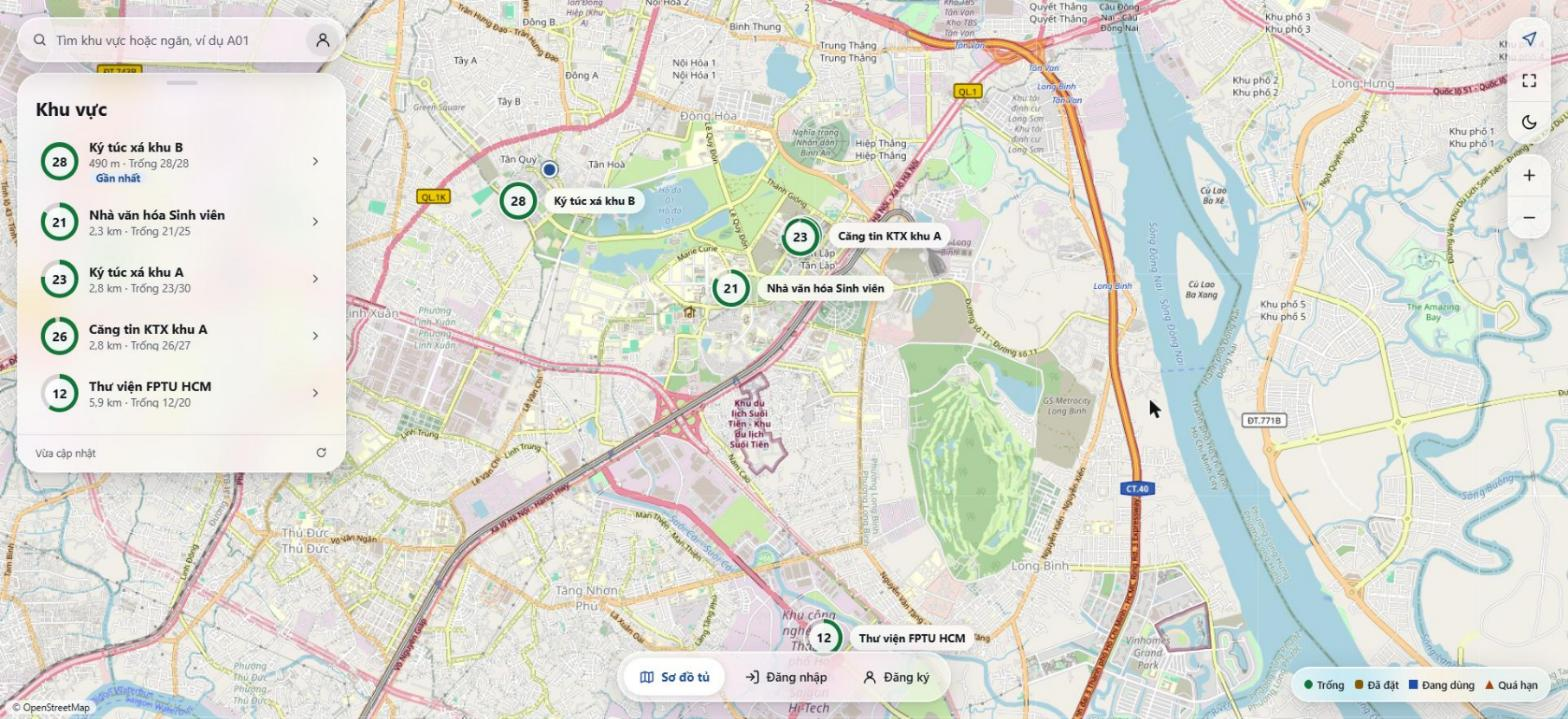
\includegraphics[width=0.48\linewidth]{images/map-visitor.png}
\hfill
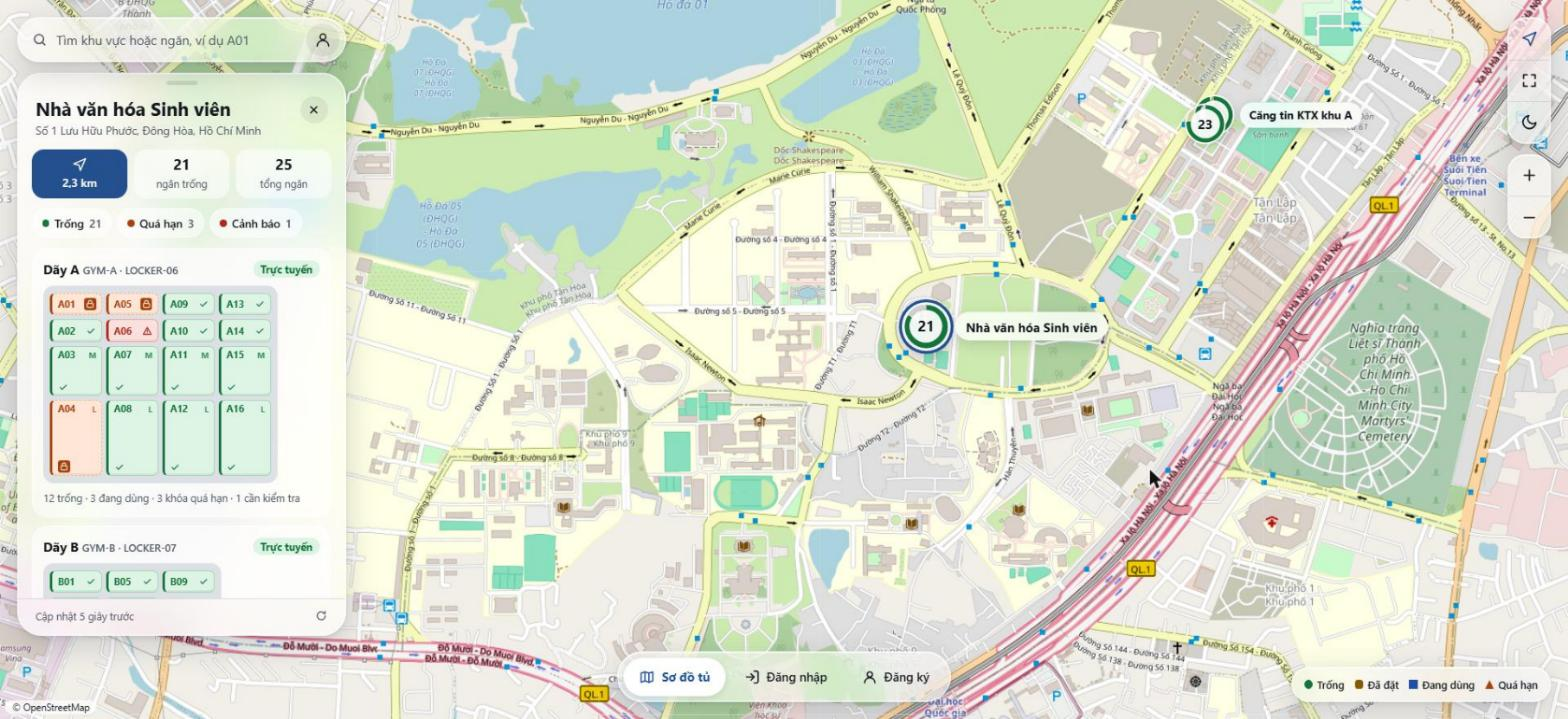
\includegraphics[width=0.48\linewidth]{images/map-area.png}\\[6pt]
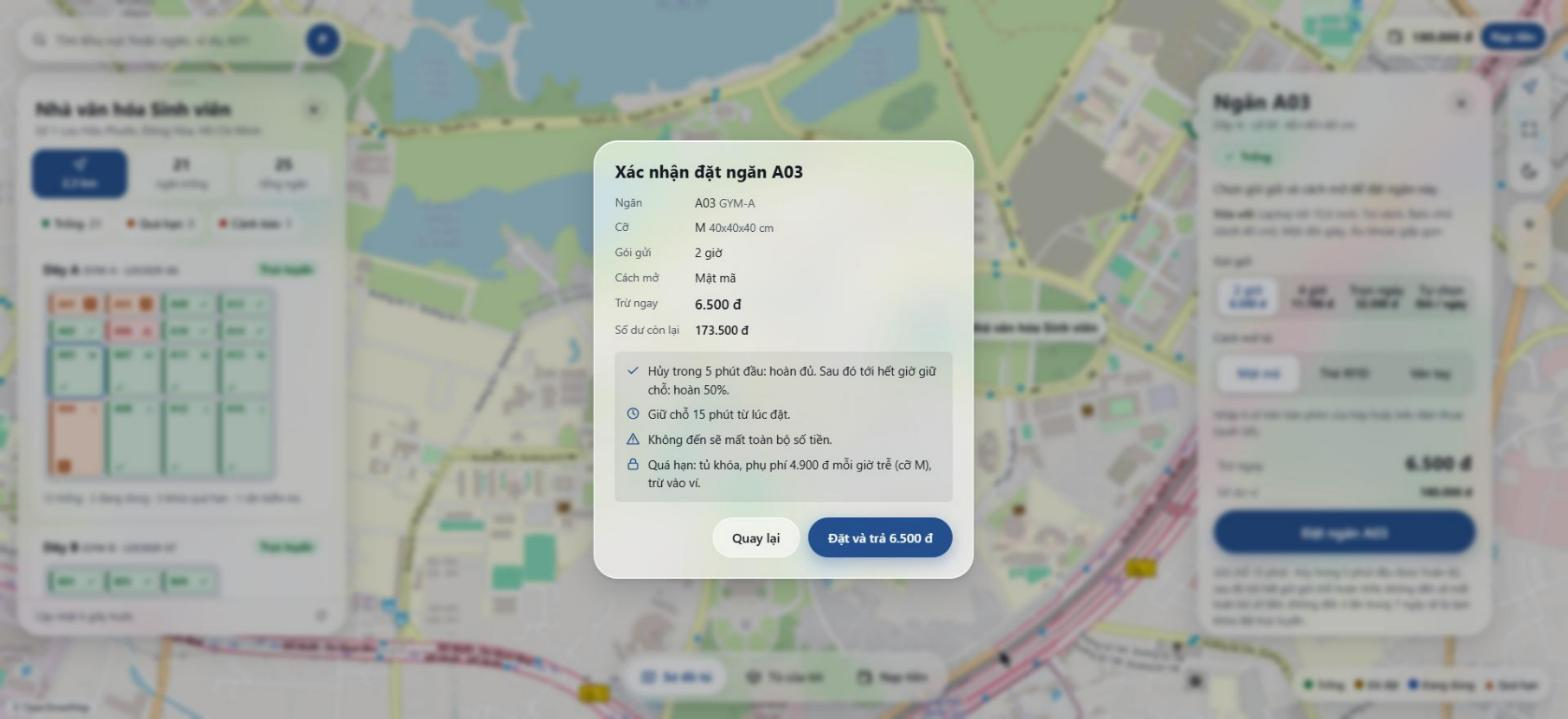
\includegraphics[width=0.48\linewidth]{images/booking-confirm.png}
\hfill
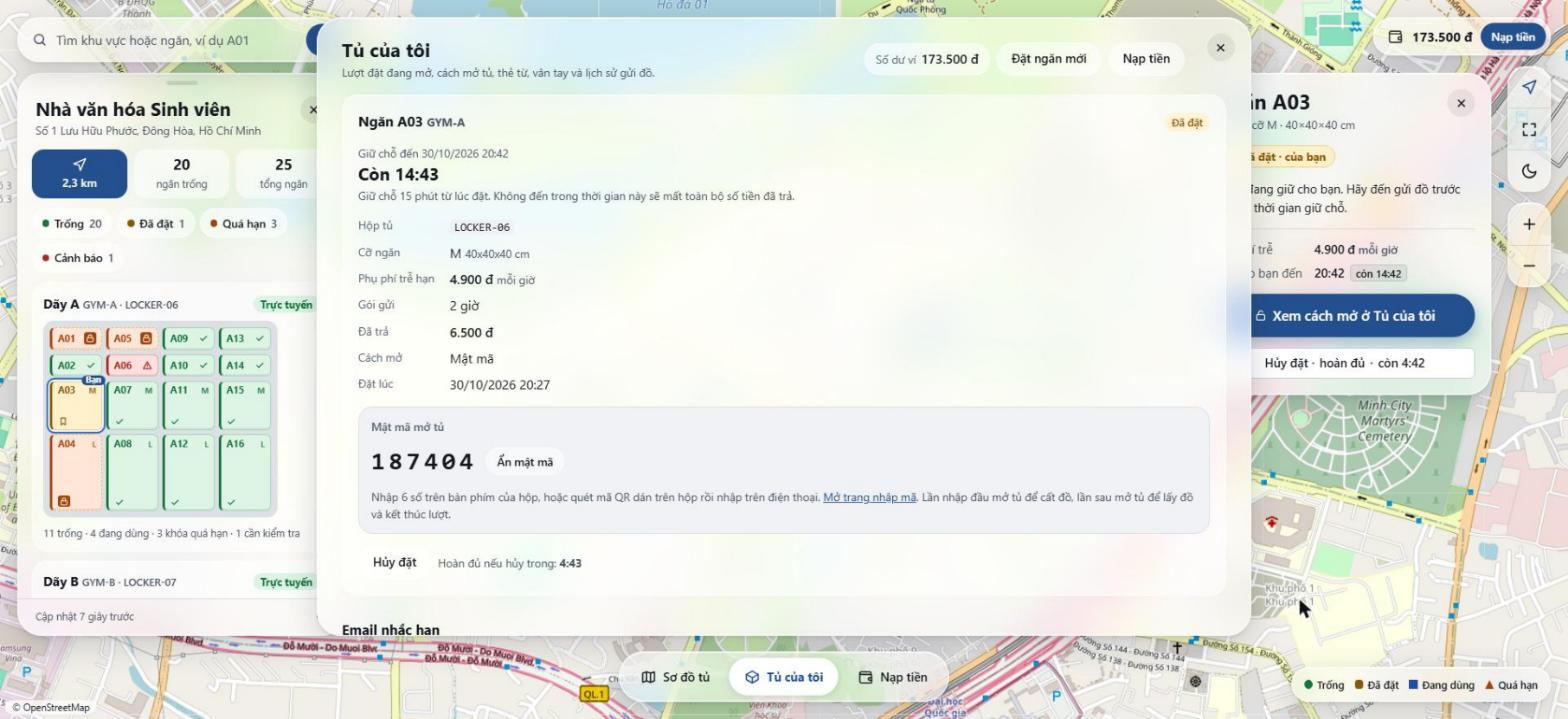
\includegraphics[width=0.48\linewidth]{images/my-locker-pin.png}
\caption{User interface (in Vietnamese): (top left) the locker map with its five areas, as seen by a visitor who is not
signed in; (top right) area GYM (``Nh\`a v\u{a}n h\'oa Sinh vi\^en''), where bank GYM-A has three overdue-locked slots and one slot with an open alert;
(bottom left) the confirmation popup for booking slot A03 of GYM-A with the 2-hour plan and a PIN; (bottom right) the
``My locker'' panel with the PIN, the hold countdown and the free-cancel countdown.}
\label{fig:ui1}
\end{figure}

\begin{figure}[H]
\centering
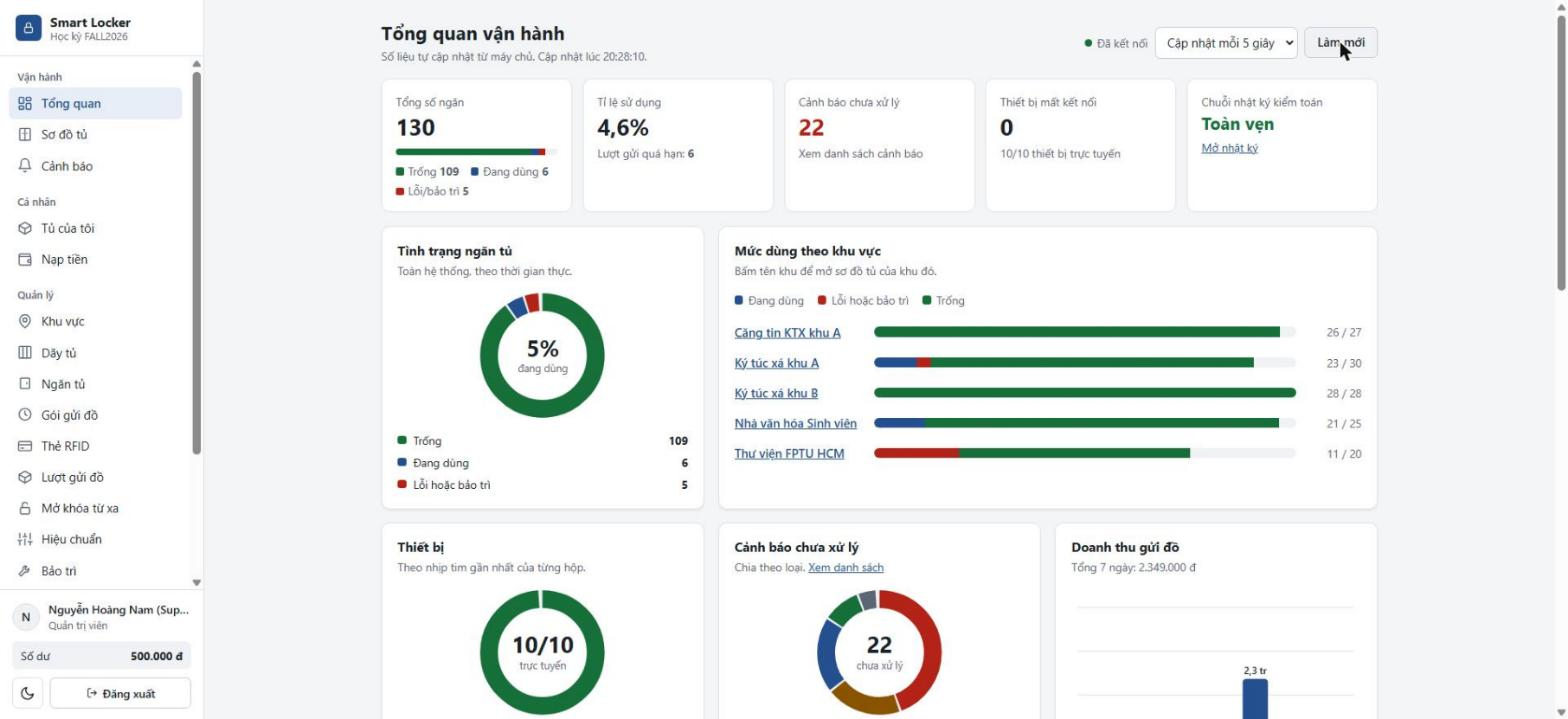
\includegraphics[width=0.48\linewidth]{images/dashboard.png}
\hfill
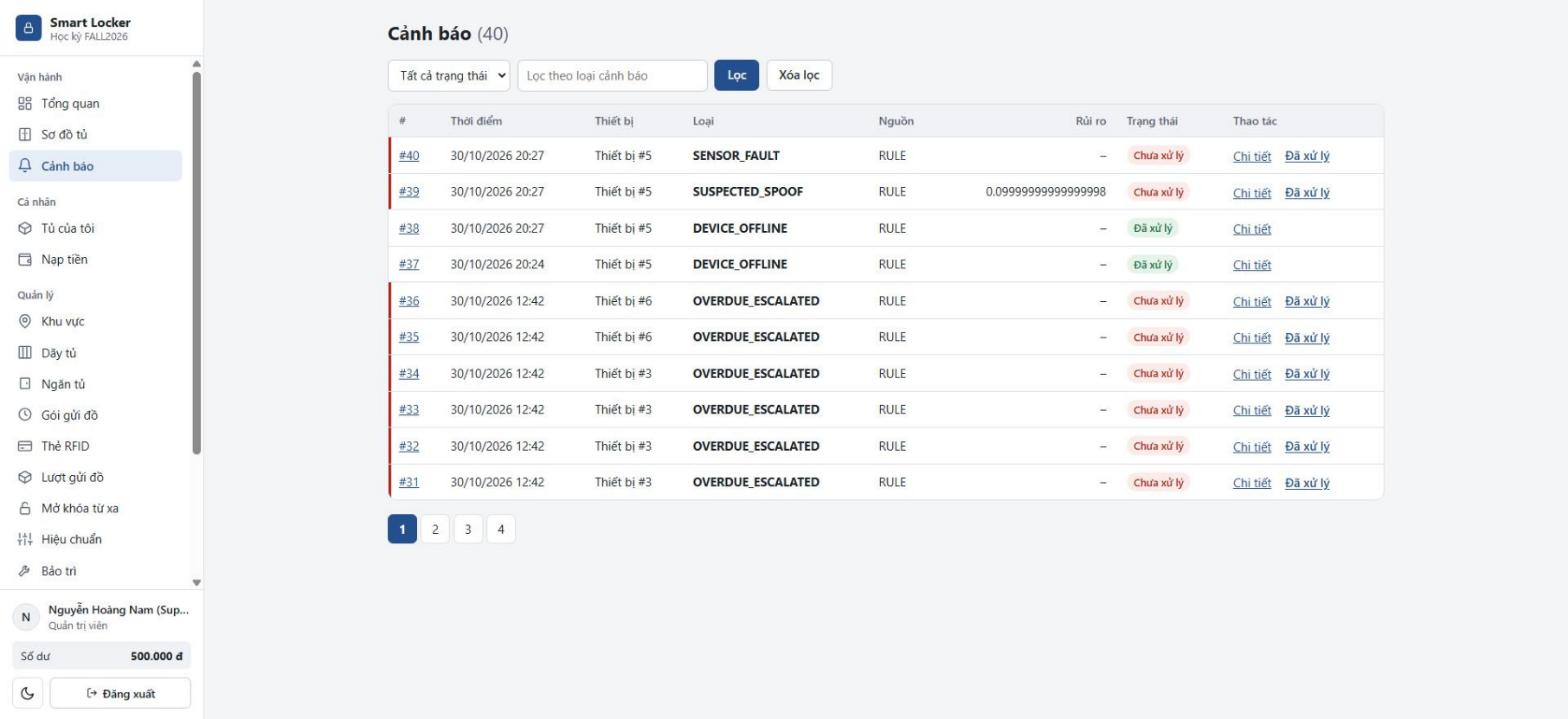
\includegraphics[width=0.48\linewidth]{images/alerts.png}\\[6pt]
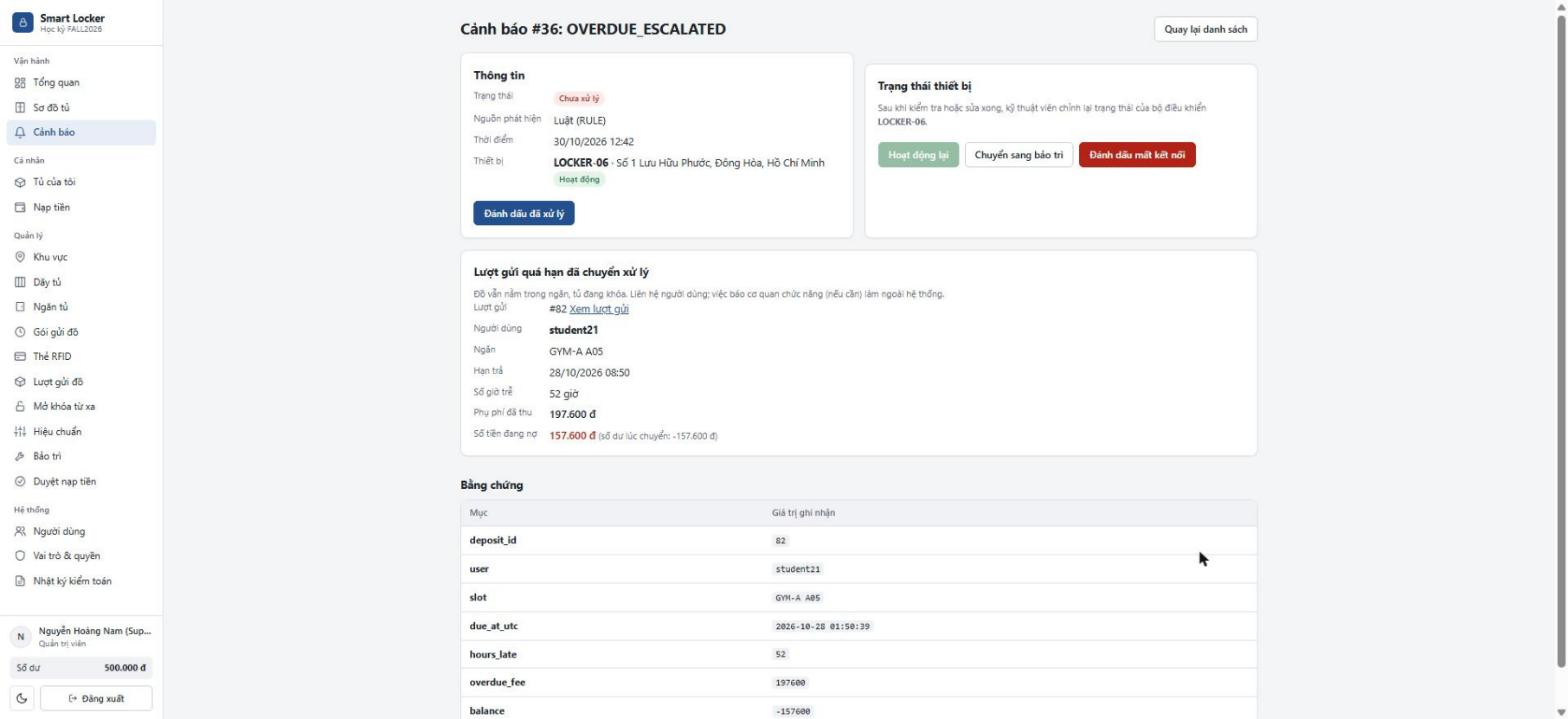
\includegraphics[width=0.48\linewidth]{images/alert-escalated.png}
\hfill
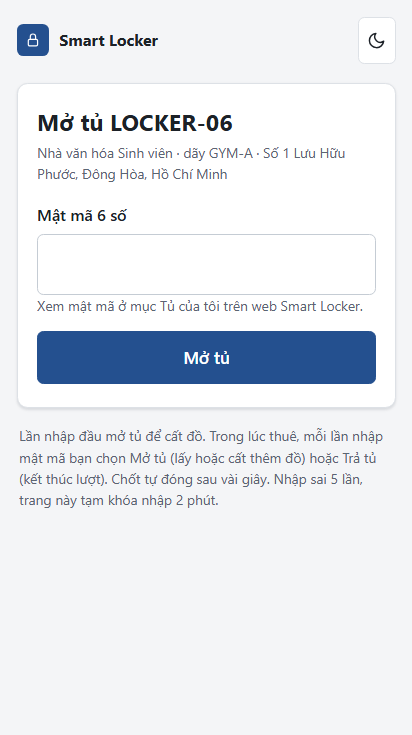
\includegraphics[width=0.25\linewidth]{images/kiosk-phone.png}
\caption{Staff and device views: (top) the staff dashboard and the alert list (all devices except LOCKER-01 are demo
devices whose heartbeat is simulated by the server); (bottom left) alert \#36, an \texttt{OVERDUE\_ESCALATED} alert for
a booking in slot A05 of GYM-A that was 52~hours late, with its evidence table; (bottom right) the phone unlock page of
box LOCKER-06 (\texttt{/k/LOCKER-06}) at phone width: a six-digit PIN field, and a note below it that explains the
5-try, 2-minute lock of the page.}
\label{fig:ui2}
\end{figure}

\section{Experimental Results and Discussion}
\label{sec:ml}

\subsection{Experimental Setup}

\textbf{Dataset.} The risk model is trained on a labelled set of 480 telemetry sessions with the five features of
Table~\ref{tab:features} and six classes (NORMAL, FORCED\_OPEN, WRONG\_USER, OVERDUE, ITEM\_LEFT, SUSPECTED\_SPOOF),
80 sessions per class. The sessions are synthetic: they are generated by the database seed script from simple
per-class patterns (e.g.\ a forced opening has no valid card, a long door time and several unlock events; an item left
behind has a positive weight change), because the prototype box has no door sensor or load cell yet. Wrong-user
sessions are generated with exactly the same formulas as normal ones, since the telemetry of a wrong user is that of a
normal visit; the two classes differ only in the row index that the formulas take as input.

\textbf{Protocol.} Four Weka classifiers were compared: Random Forest \cite{breiman2001rf}, J48 (C4.5)
\cite{quinlan1993c45}, Naive Bayes \cite{john1995nb} and IBk with $k = 5$ \cite{aha1991ibl}, otherwise with default
parameters. Each was evaluated with stratified 10-fold cross-validation \cite{kohavi1995cv} (random seed 42) in two
settings: the six-class problem, and a binary problem (NORMAL vs.\ ABNORMAL, label order \{NORMAL, ABNORMAL\}), which
measures the NORMAL-versus-rest decision that the risk score makes; the binary models are an additional analysis and
are not deployed. Training time is the median of 11 builds on all 480 sessions; inference time is averaged
over $20 \times 480$ predictions after one warm-up pass; the timing was repeated in three runs.
All experiments ran on a laptop with an Intel Core i5-11400H (2.7~GHz, 6 cores), 16~GB RAM and Windows~11 (64-bit),
using Oracle JDK 1.8.0\_202 and Weka 3.8.6; the server-side measurements of Section~\ref{sec:latency} used Tomcat
9.0.113 (on JDK 1.8.0\_171) and SQL Server 2022 on the same laptop.

\subsection{Classification Results}

\begin{table}[H]
\renewcommand{\arraystretch}{1.3}
\centering
\caption{10-Fold Cross-Validation Results (Weighted Averages)}
\label{tab:ml}
\begin{tabular}{l c c c c c c}
\hline
 & \multicolumn{4}{c}{\textbf{Six classes}} & \multicolumn{2}{c}{\textbf{Binary}} \\
\textbf{Model} & \textbf{Accuracy} & \textbf{Precision} & \textbf{Recall} & \textbf{F1} & \textbf{Accuracy} & \textbf{F1} \\
\hline
Random Forest & 0.948 & 0.949 & 0.948 & 0.948 & 0.938 & 0.939 \\
J48 (C4.5)    & 0.856 & 0.857 & 0.856 & 0.856 & 0.831 & 0.848 \\
Naive Bayes   & 0.779 & 0.778 & 0.779 & 0.778 & 0.833 & 0.852 \\
IBk ($k=5$)   & \textbf{0.977} & \textbf{0.978} & \textbf{0.977} & \textbf{0.977} & \textbf{0.975} & \textbf{0.975} \\
\hline
\end{tabular}
\end{table}

Table~\ref{tab:ml} shows that IBk obtains the best weighted F1 in both settings (0.977 and 0.975),
followed by Random Forest (0.948 and 0.939). Naive Bayes is the weakest in the six-class setting (0.778). All models
are cheap enough for online scoring: in the six-class setting Random Forest trains in about 36--38~ms and scores a
session in 12--15.5~$\mu$s, while IBk needs no real training (under 1~ms) and scores a session in 15--17~$\mu$s
(ranges over the three runs).

\begin{table}[H]
\renewcommand{\arraystretch}{1.3}
\centering
\caption{Confusion Matrix and Per-Class F1 of IBk ($k=5$), Six Classes, 10-Fold Cross-Validation}
\label{tab:cm}
\begin{tabular}{l c c c c c c c}
\hline
\textbf{Actual $\backslash$ Predicted} & \textbf{FO} & \textbf{WU} & \textbf{OD} & \textbf{IL} & \textbf{SS} & \textbf{NO} & \textbf{F1} \\
\hline
FORCED\_OPEN (FO)     & 80 & 0  & 0  & 0  & 0  & 0  & 1.000 \\
WRONG\_USER (WU)      & 0  & 73 & 0  & 0  & 0  & 7  & 0.936 \\
OVERDUE (OD)          & 0  & 0  & 80 & 0  & 0  & 0  & 1.000 \\
ITEM\_LEFT (IL)       & 0  & 0  & 0  & 79 & 1  & 0  & 0.994 \\
SUSPECTED\_SPOOF (SS) & 0  & 0  & 0  & 0  & 80 & 0  & 0.994 \\
NORMAL (NO)           & 0  & 3  & 0  & 0  & 0  & 77 & 0.939 \\
\hline
\end{tabular}
\end{table}

\subsection{Discussion}

The confusion matrix of IBk, the deployed model (Table~\ref{tab:cm}), shows where the errors
lie. Every FORCED\_OPEN, OVERDUE and SUSPECTED\_SPOOF session is classified correctly and one ITEM\_LEFT session is
labelled SUSPECTED\_SPOOF, because each abnormal class except WRONG\_USER changes at least one telemetry feature in a
distinctive way. The other 10 of the 11 errors are between WRONG\_USER and NORMAL (7 wrong-user sessions labelled
NORMAL and 3 normal sessions labelled WRONG\_USER). Random Forest shows the same pattern: all of its errors are between
these two classes (17 wrong-user sessions labelled NORMAL and 8 normal sessions labelled WRONG\_USER). This pattern is a
property of how the data is built, not an empirical finding: a valid card of another user produces the door, weight and
stay time of a normal visit, so the generator draws both classes from the same formulas. That IBk and Random Forest
still separate most wrong-user sessions is an artefact of the generator, whose formulas give the two classes slightly
different values through the row index, and should not be expected on real data. In the binary setting, Naive Bayes
classifies every normal session correctly but labels 80 of the 400 abnormal sessions as NORMAL.

The design argument does not depend on these scores. Wrong-user access is a question of \emph{identity}, which is answered exactly
by comparing the card owner with the booking owner in the rule engine (rule~5), not by telemetry. The same holds for lost
cards and for spoofed remote opens, which depend on the card status and on the command table. The learned model is
therefore used only as a secondary signal for unusual combinations of door time, weight and stay time that no rule
describes, and its alerts are marked with the source ML so that operators can treat them with more caution, in line
with \cite{sommer2010outside}.

\subsection{Functional Testing}
\label{sec:tests}

The system was tested at three levels:
\begin{itemize}
  \item \textbf{Unit and integration tests} (TestNG): 66 tests covering the rule engine (14 tests), the risk scorer,
        pricing in Java and its agreement with the SQL functions, the audit hash chain and its check on a large log, the
        device heartbeat, pick-up and bank-assignment rules in the database, password and key hashing, the e-mail
        templates, the card confirmation links and the box messages. Result: all 66 passed, none skipped, on a database
        built from the SQL scripts.
  \item \textbf{API scenarios} (Postman/newman): 18 scenarios covering PIN, phone, card and fingerprint access, a lost
        card, a PIN booking opened with a card, a PIN of a finished booking or of another box, a wrong API key or body,
        wrong codes and the 5-try lockout, no-show, overdue lock, top-up, cancel, the balance buffer, escalation,
        extension and repeated opens during one rental, plus single requests to the device endpoints. For these runs the
        test box temporarily managed two banks that both have a slot A01. The first run failed one assertion: a session
        upload (\texttt{/api/locker/batch}) in the phone scenario was answered with HTTP 500, because the server looked
        up the slot of a session by box and slot code only and found two rows. The server now resolves the slot by the
        bank code or by the slot of the session's command, and otherwise rejects the session as
        \texttt{AMBIGUOUS\_SLOT}. The run after this fix, a final run on the released build (2~min 27~s) and a later run
        after the card e-mail confirmation was added each gave 221 requests and 472 assertions with none failed. The
        collection has no step yet for \texttt{CONFIRM\_EMAIL} or \texttt{WRONG\_PLACE}.
  \item \textbf{Detection scenarios}: a device simulator sends device API requests (heartbeats, credentials and session
        uploads), authenticated with the key of the real box LOCKER-01, and the database is queried after each scenario (Table~\ref{tab:scen}).
\end{itemize}

\begin{table}[H]
\renewcommand{\arraystretch}{1.3}
\centering
\caption{Detection Scenarios Replayed through the Device API}
\label{tab:scen}
\begin{tabular}{l p{5.0cm} p{3.0cm} p{6.0cm}}
\hline
\textbf{Scenario} & \textbf{Input} & \textbf{Expected} & \textbf{Observed} \\
\hline
heartbeat & 6 heartbeats 10~s apart, then silence & DEVICE\_OFFLINE within 90--105~s & device \texttt{OFFLINE}, \texttt{DEVICE\_OFFLINE} alert 104.6~s after the last heartbeat \\
remote    & staff remote open in the web; the box reports a remote session with the command id, then replays it & STAFF\_OPEN (no alert); replay SUSPECTED\_SPOOF & first session: no alert, command \texttt{DONE} (audit \texttt{COMMAND\_DONE}); replay: \texttt{SUSPECTED\_SPOOF} \\
spoof     & remote session with a command id the server never issued & SUSPECTED\_SPOOF & \texttt{SUSPECTED\_SPOOF} (``remote open without a valid command'') \\
lostcard  & card reported lost in the web, then used at the box & LOST\_CARD\_USED & \texttt{LOST\_CARD\_USED}; the card was also in the blocked list of the heartbeat reply \\
checkin   & reservation in the web, then the booking PIN sent to \texttt{/api/device/auth} & UNLOCK, CHECK\_IN, no alert & \texttt{UNLOCK} (\texttt{CHECK\_IN}), booking \texttt{ACTIVE}, slot \texttt{OCCUPIED}, no alert \\
sensor    & session with a weight change of $-5000$~g (valid range $-200$ to 20\,000~g) & SENSOR\_FAULT, slot out of service, a ticket unless the box already has an open one & \texttt{SENSOR\_FAULT}, slot \texttt{MAINTENANCE}; no new ticket, because the box already had an open one \\
\hline
\end{tabular}
\end{table}

All six scenarios produced the expected label. Two needed a change. In the first \emph{remote} run the simulator
stamped the session with whole seconds, earlier than the command created in the same second, so both sessions were
flagged as spoofed; with a 2~s pause before the session the run above was obtained. This showed that the rule
compared the device time with the command time without any tolerance, so a device clock lagging the server caused the
same false alarm; the rule now accepts a session stamped up to 60~s before its command, and a rule-engine test covers
this window.
The simulator's own \emph{checkin} case sends only a heartbeat, which no longer checks a booking in, and left the
booking \texttt{RESERVED}; the result above was obtained by sending the booking PIN to \texttt{/api/device/auth}, as
the box does.

\subsection{Server-Side Response Time}
\label{sec:latency}

The real box was not online during the server measurements, so Table~\ref{tab:latency} reports only the \emph{server
processing time} of the device API: 30 requests per endpoint sent with curl from the same laptop, after one warm-up
request. It excludes Wi-Fi, reading the credential at the box and moving the servo. The PIN requests used the valid PIN
of an active booking with intent \texttt{ASK}, which the server answers with the ``A: open / B: return'' choice
without changing any data.

\begin{table}[H]
\renewcommand{\arraystretch}{1.3}
\centering
\caption{Server-Side Response Time of the Device API (localhost, 30 Requests Each, ms)}
\label{tab:latency}
\begin{tabular}{l c c c c c}
\hline
\textbf{Request} & \textbf{Mean} & \textbf{Median} & \textbf{p95} & \textbf{Min} & \textbf{Max} \\
\hline
Heartbeat (\texttt{/api/health})                 & 5.9  & 6.0  & 6.8  & 4.6  & 7.3 \\
PIN at the box (\texttt{/api/device/auth})       & 17.0 & 15.7 & 19.0 & 14.1 & 48.0 \\
PIN on the phone page (\texttt{/api/kiosk/unlock}) & 31.1 & 16.2 & 96.0 & 13.4 & 102.7 \\
\hline
\end{tabular}
\end{table}

All requests answered within about 0.1~s, so the time a user waits at the box is dominated by Wi-Fi, the readers and
the servo; a phone-page open additionally waits for the next heartbeat, which comes every 3~s. Two timed safeguards were
also measured. \textbf{Lockout:} wrong PINs 1 to 4 were answered with 4 down to 1 attempts left, the 5th started a
120~s lock, and during the lock even the valid PIN was refused (\texttt{LOCKED\_OUT}); the valid PIN was accepted again
at the first retry, 125.5~s after the lock started. \textbf{Offline detection:} with a 90~s timeout checked by a 15~s
job, the expected delay is 90--105~s; the heartbeat scenario measured 104.6~s, and four earlier offline alerts of the
same box in the database took 97--98~s. These four delays are computed from a last-seen time stored to the whole
second, so they may be off by up to 1~s. Of the two other earlier alerts, one took 110~s because the
application was reloaded during the wait, and one was excluded because the server was stopped during that period.

\textbf{End-to-end opening on the real box:} 20 openings from the phone page took 1.67~s on average from sending
the PIN until the door opened. This includes the wait for the box's next heartbeat (every 3~s, so 1.5~s on average),
which is therefore most of the delay; the server time above is a small part of it.

\subsection{Limitations}

The evaluation has four main limitations. First, the prototype box has no door sensor and no load cell (its ultrasonic
sensor only drives the LCD backlight), and its firmware does not upload sessions yet; every session in the experiments
comes from the device simulator or the seed data, not from measurements of the box. Second, the training data is
synthetic, its class patterns are simple and its wrong-user and normal sessions share the same formulas, so the
cross-validation scores are optimistic and do not predict performance on real lockers; a transfer test (train on the
synthetic set, test on about 100 labelled device sessions) is implemented but could not be run without real labelled
sessions. Third, only one slot of the prototype has a physical lock; the box manages a few more slots
logically, and the other banks shown in the figures belong to demo devices whose heartbeat is simulated by the server.
Fourth, the transport security of the prototype is basic: web forms carry no CSRF token (the only protection is the
\texttt{SameSite=Lax} session cookie), the box connects only over Wi-Fi, and Tomcat itself serves plain HTTP. HTTPS is
available only through a Cloudflare tunnel, and the firmware does not verify the server certificate
(\texttt{setInsecure}), so the per-device key could be intercepted on an untrusted network.

\section{Conclusion}

This paper presented SmartLocker, a smart locker rental system that combines online reservation, size-based pricing,
multiple opening methods (PIN, RFID card, fingerprint, phone) and an ESP32 box that delegates every decision to the
server. Anomalous access is detected in two tiers: a priority-ordered rule engine that uses device telemetry together
with server context, and a machine-learning risk score that adds evidence and covers cases no rule describes.
Operational safeguards (a 120~s lockout after five wrong guesses, offline detection within 90--105~s while the server
runs, overdue lock and 48-hour escalation) and a hash-chained audit log complete the design.

On 480 synthetic, labelled sessions, IBk reached a weighted F1 of 0.977 and Random Forest 0.948 in 10-fold
cross-validation. Most of their errors are between wrong-user and normal sessions, which the data generator builds from
the same formulas; this illustrates, rather than proves, that identity checks belong in explicit rules and that the
learned model is best used as a supporting signal. The system passed all 66 unit and integration tests and all 472
assertions of the 18 API scenarios; the six detection scenarios replayed through the device API produced
the expected labels (two after adjusting the simulator), and on localhost the server processed device requests in a
mean time of 6--31~ms per endpoint.

Future work includes adding a reed switch and a load cell to the box and uploading its sessions, so that door and
weight telemetry come from real sessions, collecting and labelling real sessions to train and evaluate the model on real data, measuring the
end-to-end time of the keypad, card and fingerprint openings on the box, extending the prototype to several physically locked slots, and adding CSRF
tokens and certificate verification on the box.

\bibliographystyle{IEEEtran}
\bibliography{references}

\end{document}
